\documentclass[10pt,twocolumn,letterpaper]{article}

% Add necessary BibTeX commands
% \usepackage{cite} % Add this line to handle citations

% \bibliographystyle{ieee_fullname}

%%%%%%%%% PAPER TYPE  - PLEASE UPDATE FOR FINAL VERSION
%\usepackage[review]{cvpr}      % To produce the REVIEW version
\usepackage{cvpr}              % To produce the CAMERA-READY version
%\usepackage[pagenumbers]{cvpr} % To force page numbers, e.g. for an arXiv version
\usepackage{graphicx}
\usepackage[ruled, vlined]{algorithm2e}
\usepackage{amsmath}
\usepackage{booktabs}
\usepackage[pagebackref,breaklinks,colorlinks]{hyperref}
\usepackage{algorithm2e}
\usepackage{lipsum}


% Support for easy cross-referencing
\usepackage[capitalize]{cleveref}
\crefname{section}{Sec.}{Secs.}
\Crefname{section}{Section}{Sections}
\Crefname{table}{Table}{Tables}
\crefname{table}{Tab.}{Tabs.}


\newcommand{\cvprPaperID}{27191964} % *** Enter the CVPR Paper ID here
\newcommand{\confName}{CVPR}
\newcommand{\confYear}{2023}

\begin{document}
    \title{LiDAR-DenseSeg: A Framework for Aerial LiDAR Semantic Segmentation, Densification, and Planar Flattening for Improved Voxelization and Mesh Reconstruction}
    \author{Ashtan Mistal\\
    University of British Columbia
    }

    \maketitle

    % Write a maximum of six-page document (excluding citations, not a hard limit if you need more space) in the CVPR format.

    \begin{abstract}
        This paper introduces LiDAR-DenseSeg, a novel framework designed to enhance voxelization and mesh reconstruction of airborne LiDAR data. The process involves three pivotal steps: Semantic segmentation, densification, and planar flattening of the point cloud. Using a modified PointNet++ architecture, the framework effectively segments point cloud data, focusing primarily on building structures and achieving an evaluation accuracy of 94.1\% and a mean IoU of 0.89.
        Following segmentation, a recursive median split algorithm based on the SAPCU architecture densifies the point cloud, addressing the inherent sparsity in airborne LiDAR data. Planar flattening is proposed to further refine the process, reducing noise and enhancing voxelization quality. The paper presents empirical results demonstrating significant improvements in the voxelization and mesh reconstruction of airborne LiDAR data, contributing to the field of LiDAR data processing and 3D reconstruction.
        Code is available at \url{https://github.com/ashtanmistal/LiDAR-DenseSeg}.
\end{abstract}

    \section{Introduction}\label{sec:introduction}

    Voxelization and mesh reconstruction of airborne LiDAR data inherently suffers from numerous issues, including but not limited to: (1) the lack of complete semantic labels, (2) the sparsity of the data, and (3) the irregularity of the point cloud.
    A naive approach of voxelization leads to poor reconstruction quality and an inability to capture the fine details of the point cloud\cite{MinecraftUBC}.
    Lack of complete labels leads to the direct voxelization not being a complete representation of the available point cloud data, and entire sections of the point cloud being lost in the voxelization process due to a lack of labels.
    The irregularity of the point cloud leads to neighbouring points that lie along a plane in the real world to be mapped to different voxels, leading to massive amplification of noise if the voxelization is performed naively.
    The sparsity of the data leads to the voxelization and mesh reconstruction processes being unable to capture the fine details of the point cloud.
    This paper proposes a framework for improving the voxelization and mesh reconstruction of airborne LiDAR data by first semantically segmenting the point cloud, then densifying the point cloud, and finally performing planar flattening on the densified point cloud.

    \begin{figure*}
        \centering
        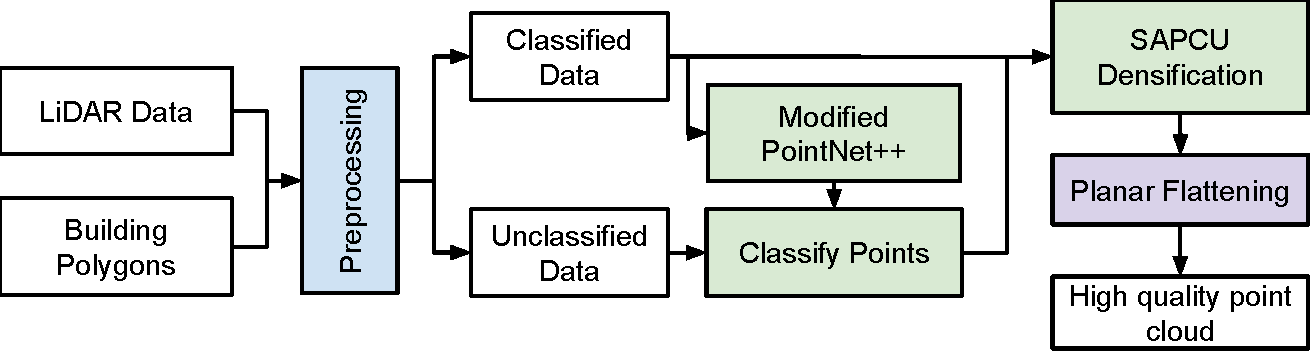
\includegraphics[width=\linewidth]{533Y Model Pipeline.pdf}
        \caption{The LiDAR-DenseSeg pipeline. Data streams are in white, data processing is in blue, deep learning tasks are in green, and mesh processing is in purple. The high quality point cloud is the output of the pipeline.}
        \label{fig:pipeline}
    \end{figure*}

    The semantic segmentation of the point cloud is performed using a PointNet++ architecture~\cite{qi2017pointnet} that is trained on the already labelled data.\
    The data is a partially labelled point cloud of the University of British Columbia campus, with the main labels of buildings, trees, water, and ground.
    This framework focuses on labelling buildings, as these are the most important features to capture in the voxelization and mesh reconstruction process and the ones that suffer the most from the aforementioned issues.
    The semantic segmentation problem is thus formulated as a binary problem, with the two classes being \textit{buildings} and \textit{not buildings}.

    The densification of the point cloud is performed using a recursive median split implementation of the SAPCU architecture~\cite{sapcu} using pre-trained weights from the authors.
    A weighted nearest neighbours algorithm is used to transfer the colour information from the original point cloud to the densified point cloud.
    The densification task is performed only on the buildings, and primarily enhances mesh reconstruction of the buildings given the large voxel size in the voxelization process.

    To resolve the issue of the irregularity of the point cloud and fix the amplification of noise that occurs during the voxelization process, planar flattening is performed on the densified point cloud.
    For points that lie on a plane, they are brought to the plane along their normal.
    As a result, points are much more likely to get voxelized to the same voxel as their neighbours.
    This leads to a massive reduction in the noise of the point cloud, and an increase in voxelization quality.

    We present the following contributions:
    \begin{itemize}
        \item A framework for improving the voxelization and mesh reconstruction of airborne LiDAR data.
        \item A trained PointNet++ architecture for semantically segmenting buildings in airborne LiDAR data.
        \item A recursive median split implementation of the SAPCU architecture for densifying arbitrary-size and arbitrary-scale point clouds.
        \item Implementation of planar flattening for reducing noise in the voxelization process.
        \item Empirical results showing the effectiveness of the proposed framework in improving the input point cloud for voxelization and mesh reconstruction.
        \end{itemize}

        

    \section{Related Work}\label{sec:related-work}

    \textbf{MinecraftUBC.} LiDAR-DenseSeg is built on top of the MinecraftUBC~\cite{MinecraftUBC} project, which is a proof-of-concept for voxelization of airborne LiDAR data into a Minecraft world.
    The voxelization was done in a layered approach.
    The first layer was surface reconstruction of the ground data, which was done using a flood-fill algorithm.
    This was the colorized using a pre-existing GeoJSON dataset denoting ground information.
    The buildings were then placed using direct voxelization of the building data using truncation to the nearest voxel.
    Additional GeoJSON data was used to place trails, traffic impactors, and other similar features.
    Trees were then placed using a combination of direct voxelization and mean shift clustering for trunk placement.
    This work utilizes the same dataset as MinecraftUBC, and builds on top of the naive building reconstruction algorithm used in MinecraftUBC\@.
    Ultimately, the building reconstruction algorithm used in MinecraftUBC suffered from numerous problems, including but not limited to: (1) the lack of complete semantic labels, (2) the sparsity of the data, and (3) the irregularity of the point cloud.
    This meant that quality buildings had to be manually edited and colorized, and the voxelization process was unable to capture the fine details of the point cloud.
    It is thus used as a baseline for comparison in the evaluation of LiDAR-DenseSeg.

    \textbf{PointNet++ Architecture.} The PointNet++ architecture~\cite{qi2017pointnet} is a deep learning architecture for point cloud classification and segmentation that is built on top of the PointNet architecture.
    It utilizes local point features and global point features to classify and segment point clouds.
    Pre-trained (and readily available) models in PyTorch related to building semantic segmentation are few and far between, and so a PointNet++ architecture is trained on the available building data of the UBC campus.

    \textbf{SAPCU Architecture.} The SAPCU architecture~\cite{sapcu} is a deep learning architecture for self-supervised arbitrary-scale point cloud upsampling that utilizes an implicit neural representation to upsample point clouds.
    The model is trained on a normalized watertight subset of ShapeNet~\cite{chang2015shapenet, Occupancy_Networks} and based off of Occupancy Networks~\cite{Occupancy_Networks} and DGCNN~\cite{dgcnn}.
    Though the model is trained on watertight point clouds, it is able to generalize to other point clouds including non-watertight point clouds~\cite{sapcu}.
    A drawback of the model is that it is unable to perform effectively on large point clouds due to implementation limitations.
    Additionally, the model is unable to transfer colour information from the original point cloud to the densified point cloud.

    \section{Methodology}\label{sec:methodology}

    Given a partially labelled point cloud and 2d polygons for building footprints, LiDAR-DenseSeg reconstructs buildings in the input aerial LiDAR point cloud through a three-step process: (1) semantic segmentation, (2) densification, and (3) planar flattening.
    The pipeline outlined in Figure~\ref{fig:pipeline} is used to perform this task.

    

    \subsection{Preprocessing}\label{subsec:preprocessing}

    The original LiDAR data comes separated as square kilometre tiles.
    This sometimes leads to buildings being split across multiple tiles, and so the tiles are merged together to form a single point cloud.
    This single point cloud is then filtered into points that lie within a 5m radius of the building footprints, reducing the dataset size from 40~GB to 3.8~GB\@.
    These footprints are gathered from a GeoJSON dataset~\cite{ubcgeospatial} that contains the building footprints of the University of British Columbia campus, along with corresponding information regarding their name, construction status, height, and other similar information.
    Data related to under-construction buildings are not considered for the purposes of this project, and so the corresponding footprints and related points are removed from the dataset.
    Lastly, the color data associated with the dataset is quantized to the 0-255 range (from the 0-65535 range) to reduce size, and each building is saved as a separate file in the .npy format after the final data processing tasks performed in the dataloaders.

    \subsection{Semantic Segmentation}\label{subsec:semantic-segmentation}

    \begin{figure}
        \centering
        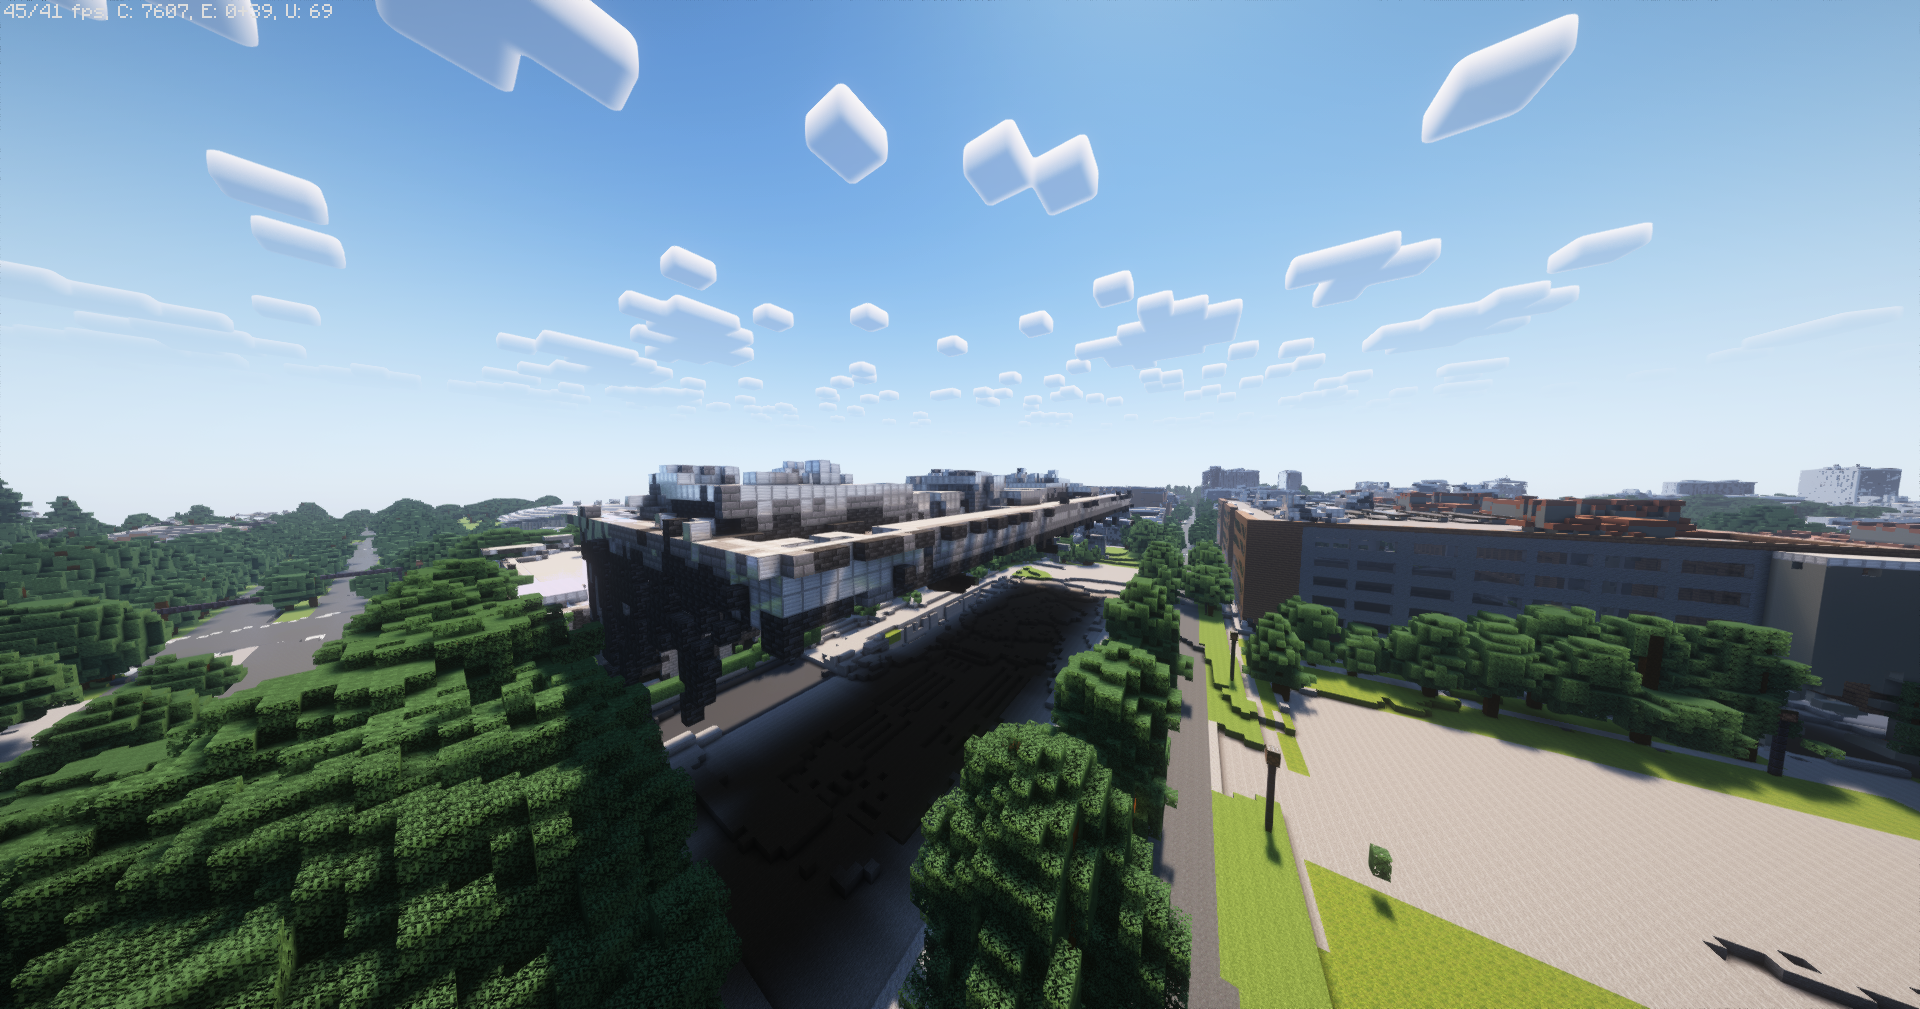
\includegraphics[width=\linewidth]{naive_voxelization.png}
        \caption{The naive voxelization of the point cloud. The lack of complete labels leads to the voxelization not being a complete representation of the available point cloud data, and entire sections of the point cloud being lost in the voxelization process due to a lack of labels. Here, every single wall in the Pharmeceutical Sciences building is not captured in the voxelization.}
        \label{fig:naive_voxelization}
    \end{figure}

    The points already labelled as buildings in the input point cloud do not cover significant regions of some buildings, and the quality of the reconstruction is significantly hindered by the lack of complete labels as seen in Figure~\ref{fig:naive_voxelization}.
    This data is present in the dataset, but is not labelled.
    The semantic segmentation task is to train a model to segment points belonging to buildings, and apply the model to the unclassified data in the point cloud.
    This is done using a modified PointNet++ architecture~\cite{qi2017pointnet} that is trained on the labelled data.
    The modifications and additions made in the PointNet++ architecture are as follows:

    \textbf{KNN Fallback in Ball Query.} The ball query in the PointNet++ architecture is modified to fallback to a KNN query if the number of points in the ball query is less than a threshold.
    This is due to the extreme sparsity in some areas of the data, where the ball query is unable to find enough existing points within the ball to extrapolate the local features.
    Selecting less points during the training process mitigates this issue, but lower number of points leads to a lower quality of the classification.
    As a result this fallback ensures the model can still perform well in these areas by extending the context as needed.

    \textbf{DataLoader.} A dataloader is implemented to load the data from the dataset and perform data augmentation.
    To ensure ease of use with other datasets and avoid manual overhead, the dataloader implements some later pre-processing tasks of the data. 
    Buildings that are underground or otherwise have a total height of less than 3m are removed from the dataset.
    The dataset is then split into points that are already classified (used for training and testing) and points that are unclassified (where we apply the learned model).
    Lastly, the LiDAR data is by default in the EPSG 26910 coordinate system; we offset the data to be zeroed on the UBC campus, and apply a rotation matrix that aligns the coordinate system with UBC's roads instead of true north.
    These are the same transformations that were applied in the MinecraftUBC project~\cite{MinecraftUBC}.

    Upon initialization, the dataloader loads the data from the dataset and performs data augmentation.
    The label weights are calculated using equation~\ref{eq:label_weights}.
\begin{equation}
    \label{eq:label_weights}
    w_j = \frac{(\max(f) / f_j)^{\frac{1}{3}}}{\sum_{k=1}^{n} (\max(f) / f_k)^{\frac{1}{3}}}, \quad j = 1, \dots, n
\end{equation}
Here, \( w_j \) is the weight for class \( j \), \( f_j \) is the relative frequency of class \( j \), \( \max(f) \) is the maximum relative frequency among all classes, and \( n \) is the number of classes.
Given weights are not able to be calculated when using the model on unlabelled data, the weights are calculated using the labelled data and then passed to the model when using the model on unlabelled data.


    \textbf{Training.} The model is trained on the labelled data using the Adam optimizer with an initial learning rate of 0.01, a batch size of 32, a weight decay of 0.0001, and a learning rate scheduler that reduces the learning rate by a factor of 0.7 every 10 epochs.
    Each building is passed individually to the model, and the centroid is calculated through a random sampling that ensures sufficient points in the block.
    The block is then centered on the centroid in the $x$ and $y$ axes, and the minimum height of the block is set to the minimum height of the building.
    The data is normalized, and both the normalized and non-normalized data is passed to the model.

    With the exception of the KNN fallback in the ball query, the rest of the PointNet++ architecture is left unchanged and used mostly as a black box.
    The model is trained on the labelled data, and then applied to the unclassified data to segment the buildings.

    A block size of 32.0m is used for the semantic segmentation, which aims to capture sufficient points in the block while ensuring applicability to smaller buildings without relying on the KNN fallback.
    4096 points are sampled from each block.
    The training is split into 70\% training data and 30\% evaluation data, and the model is trained for 64 epochs.

    \subsection{Densification}\label{subsec:densification}

    The classified point cloud is then improved further through densification.
    The model used for densification is based on SAPCU~\cite{sapcu}, which is a deep learning architecture for self-supervised arbitrary-scale point cloud upsampling that utilizes an implicit neural representation to upsample point clouds.
    Upsampling point clouds is performed with the goal of solving the problem of sparse point clouds, which is inherent in airborne LiDAR data.
    Voxelization without this task performed leads to poor reconstruction quality and an inability to capture the fine details of the point cloud, as seen in Figure~\ref{fig:walter_gage_minecraftubc}.

    \begin{figure}
        \centering
        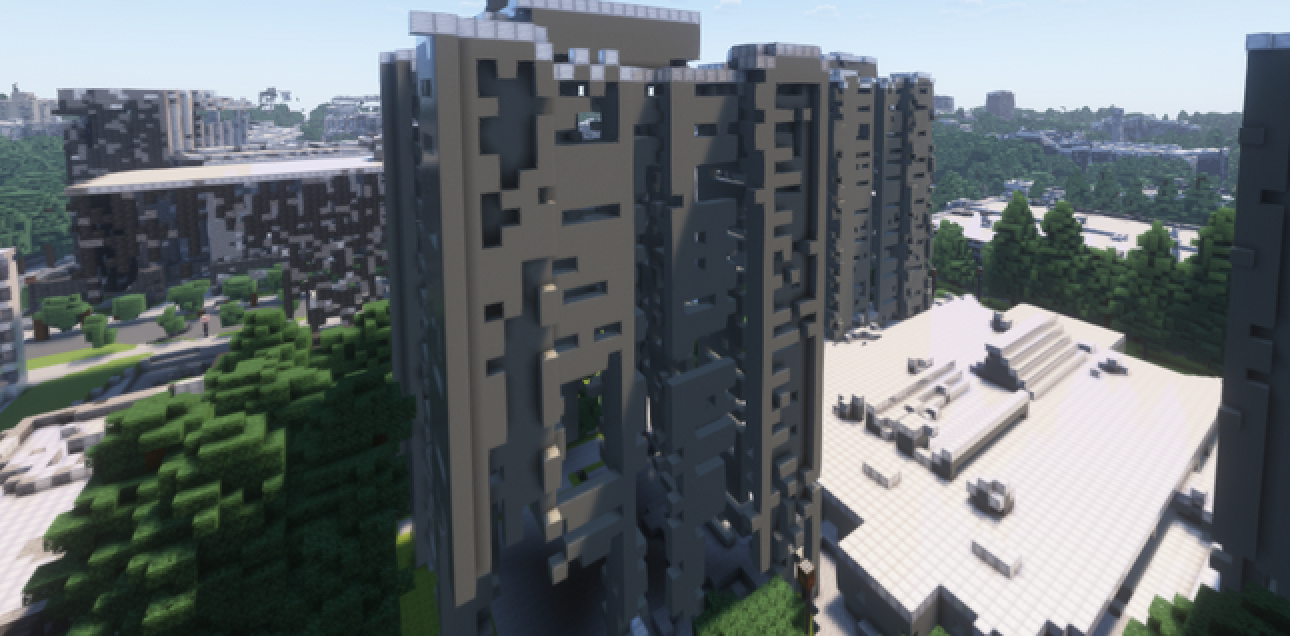
\includegraphics[width=\linewidth]{Walter_Gage.png}
        \caption{The Walter Gage residence reconstructed using the naive voxelization algorithm used in MinecraftUBC. Note the lack of detail in the deck on a per-floor basis caused by the sparsity of the data.}
        \label{fig:walter_gage_minecraftubc}
    \end{figure}

    In order to upsample the point cloud, we aim to address some of the limitations of the SAPCU architecture.
    Most notably, the SAPCU architecture is unable to perform effectively on large point clouds due to implementation limitations.
    Simply increasing the size of the KDTree used in the model does not solve this issue, as the size remains fixed and unable to adapt to variable point cloud sizes.
    Additionally, increasing this size leads to errors in the model with a lower number of points.
    As a result, the model is unable to upsample the entire point cloud at once.
    We thus implement a recursive median split algorithm that splits the point cloud into smaller chunks, densifies each chunk, and then merges the chunks back together.

    The split is based on the median of the point cloud along the largest dimension, which is determined by the bounding box of the point cloud.
    The recursive algorithm is called with each split until the number of points in the point cloud is less than a threshold, which is 5000 as per the original implementation of the SAPCU architecture.
    In the base case of less than 5000 points, the data is normalized and passed to the model, and then re-scaled to the original size.
    The pseudo-code for the recursive median split algorithm is shown in Algorithm~\ref{alg:recursive-median-split}.

    \begin{algorithm}
        \caption{Recursive Median Split Algorithm}\label{alg:recursive-median-split}
        \DontPrintSemicolon
        
        \SetKwFunction{FMain}{recursiveMedianSplit}
        \SetKwProg{Fn}{Function}{:}{}
        \Fn{\FMain{pointCloud}}{
            \uIf{\textup{len}(pointCloud) $< $100}{
                \KwRet pointCloud\;
            }
            \uElseIf{\textup{len}(pointCloud) $<$ 5000}{
                pcN $\leftarrow$ normalize(pointCloud)\;
                pcN $\leftarrow$ SAPCU(pcN)\;
                pc $\leftarrow$ rescale(pcN)\;
                \KwRet pc\;
            }
            \Else{
                bbox $\leftarrow$ getBoundingBox(pointCloud)\;
                splitDimension $\leftarrow$ getLargestDimension(bbox)\;
                median $\leftarrow$ getMedian(pointCloud, splitDimension)\;
                left, right $\leftarrow$ split(pointCloud, median, splitDimension)\;
                left $\leftarrow$ \FMain{left}\;
                right $\leftarrow$ \FMain{right}\;
                \KwRet merge(left, right)\;
            }
        }
        \end{algorithm}
    

    The preprocessing tasks performed in this algorithm are simply that of handling the .obj files that the semantic segmentation task outputs, and selecting only the points that are classified as buildings.

    \subsection{Planar Flattening}\label{subsec:planar-flattening}

    In order to resolve the issue of the irregularity of the point cloud and fix the amplification of noise that occurs during the voxelization process, planar flattening is performed on the densified point cloud.
    For points that lie on a plane, they are brought to the plane along their normal.
    To determine what points lie on a plane, a plane detection algorithm is used.
    A point is selected at random from the unseen points, and a plane is fit to the point and its $k$ nearest neighbours.
    This plane fit is performed using a 3D RANSAC algorithm.
    If the plane is a good fit, then $k$ is increased and the plane is fit again using these new points. 
    Whether or not a plane is a good fit is determined by the number of points that lie within a threshold distance of the plane.
    If the plane is not a good fit, the next smallest plane that was a good fit is selected and the points marked as seen.
    This process is repeated until all points are seen.
    Once all points are seen, the points that lie on a plane are brought to the plane along their normal.

    The pseudo-code for the plane detection algorithm is shown in Algorithm~\ref{alg:plane-detection}.

    \begin{algorithm}
        \caption{Plane Detection Algorithm}\label{alg:plane-detection}
        \DontPrintSemicolon
        
        \SetKwFunction{FMain}{planeDetection}
        \SetKwProg{Fn}{Function}{:}{}
        \Fn{\FMain{pointCloud, threshold}}{
            unseen $\leftarrow$ pointCloud\;
            planes $\leftarrow$ []\;
            \While{\textup{len}(unseen) $>$ 0}{
                point $\leftarrow$ randomChoice(unseen)\;
                k $\leftarrow$ 3\;
                initNeighbours $\leftarrow$ getNeighbours(point, k)\;
                prevPlane $\leftarrow$ fitPlane(initNeighbours)\;
                \Repeat{length of plane $\leq$ threshold}{
                    neighbours $\leftarrow$ getNeighbours(point, k)\;
                    plane $\leftarrow$ fitPlane(neighbours)\;
                    \uIf{\textup{len}(plane) $>$ threshold}{
                        k $\leftarrow$ k + 1\;
                        prevPlane $\leftarrow$ plane\;
                    }
                    \Else{
                        append(planes, prevPlane)\;
                        remove(unseen, prevPlane.points)\;
                    }
                }
            }
            \KwRet planes\;
        }
        \end{algorithm}
    

    Once all points are fit to a plane, only planes with $n$ points or greater are considered; smaller planes are either corners, edges, or other non-planar features.
    The points that lie on these planes are then brought to the plane along their normal.
    This is done by calculating the distance from the point to the plane, and then moving the point along the normal by that distance.

    \section{Results}\label{sec:results}

    \subsection{Semantic Segmentation}\label{subsection:semantic-segmentation-results}
% Learning rate:0.001176
% BN momentum updated to: 0.010000
    \textbf{Quantitative Results.} After 64 epochs, the model achieves an evaluation accuracy of 94.1\%, with a mean IoU of 0.89. The IoU for non-buildings was 0.894, and the IoU for buildings was 0.880.
    The best model was the one in the final epoch; the learning rate was 0.001176 and the batch norm momentum was 0.01.

    We compare the results of our model that of the D-FCN model~\cite{dfcn}, which is a multi-class algorithm trained on the data fusion 2019 dataset~\cite{2019DataFusionContest}, which is a dataset of aerial LiDAR data.
    We also compare our results to a PointNet++ model also trained on the data fusion 2019 dataset.
    The results of our model are comparable to but worse than the results of the D-FCN model, which achieves an overall accuracy of 95.6\%.
    However, our model outperforms the PointNet++ multiclass model mentioned in the D-FCN paper, which achieves an overall accuracy of 92.7\%.
    This shows the effectiveness of a binary segmentation model in the context of improving building reconstruction quality.

    Additionally, further hyperparameter tuning could be performed to improve the results of the model through a grid search or similar method.
    With those improvements in mind a better comparison to the D-FCN model could be made.
    We leave these opportunities for future work and rather present this as a proof-of-concept for the effectiveness of a binary segmentation model in the context of improving building reconstruction quality.

    \textbf{Qualitative Results.} The results of the segmentation task are shown in Figure~\ref{fig:initial-segmentation-results}.
    Overall, the model does an excellent job of semantically segmenting medium-sized buildings and smaller. Most of the incorrectly classified points are speckle noise; noise that would get ignored in the voxelization process given that the voxelization considers the most common label in the block~\cite{MinecraftUBC}.
    

    \begin{figure}
        \centering
        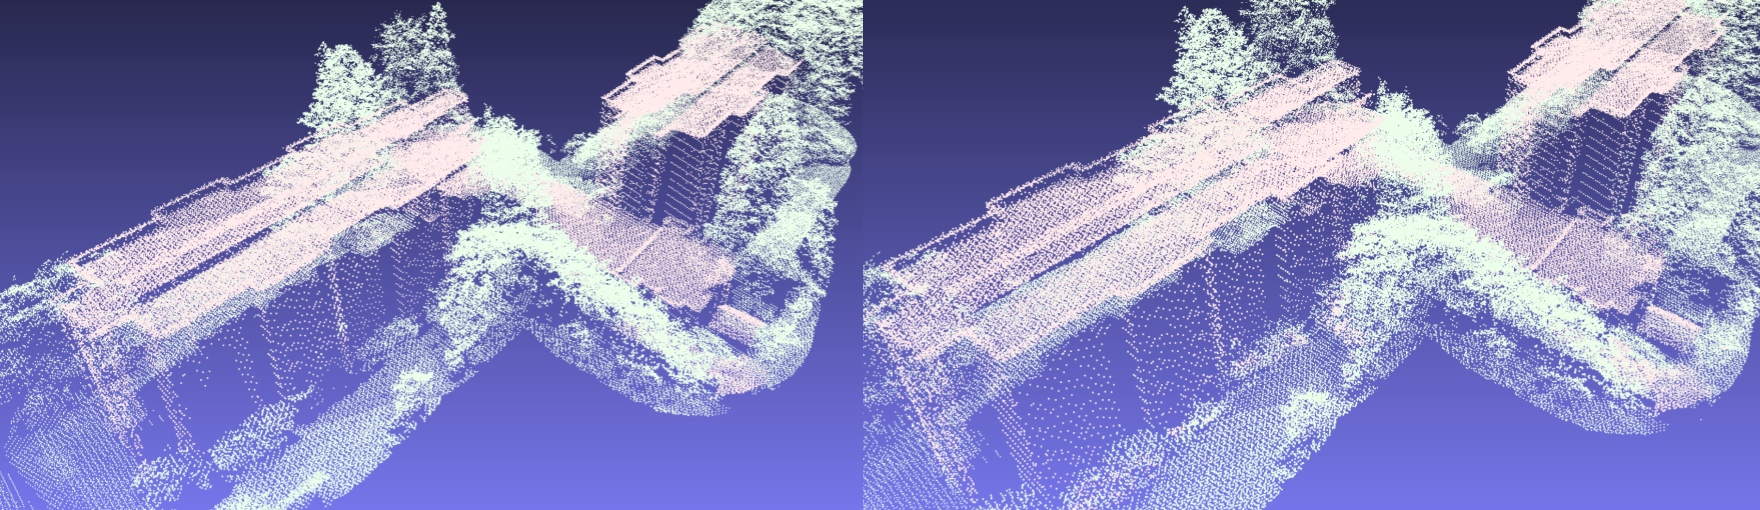
\includegraphics[width=\linewidth]{initial_classification.png}
        \caption{Top: Ground truth segmentation of buildings (red) and non-buildings (green). Bottom: Semantic Segmentation of buildings (red) and non-buildings (green) by the model. The model fills in gaps in the building walls where data is available.}
        \label{fig:initial-segmentation-results}
    \end{figure}

    When performing the model on only the unclassified data, the model is still able to segment the buildings with a high degree of visual accuracy.
    With the entire point cloud considered, the model performs even better and the additional context leads to a better result.
    Additionally, the model effectively solves the problem of missing walls in the voxelization process, as seen in Figure~\ref{fig:full-segmentation-results}.
    This greatly improves the reconstruction quality of the buildings, as the voxelization process is able to capture the entire building and not just the parts that are labelled.
    While further improvements to the model through hyperparameter tuning could still be made to improve the segmentation accuracy, the model is already able to capture the vast majority of the buildings in the point cloud and improve the reconstruction quality of the buildings.

    \begin{figure}
        \centering
        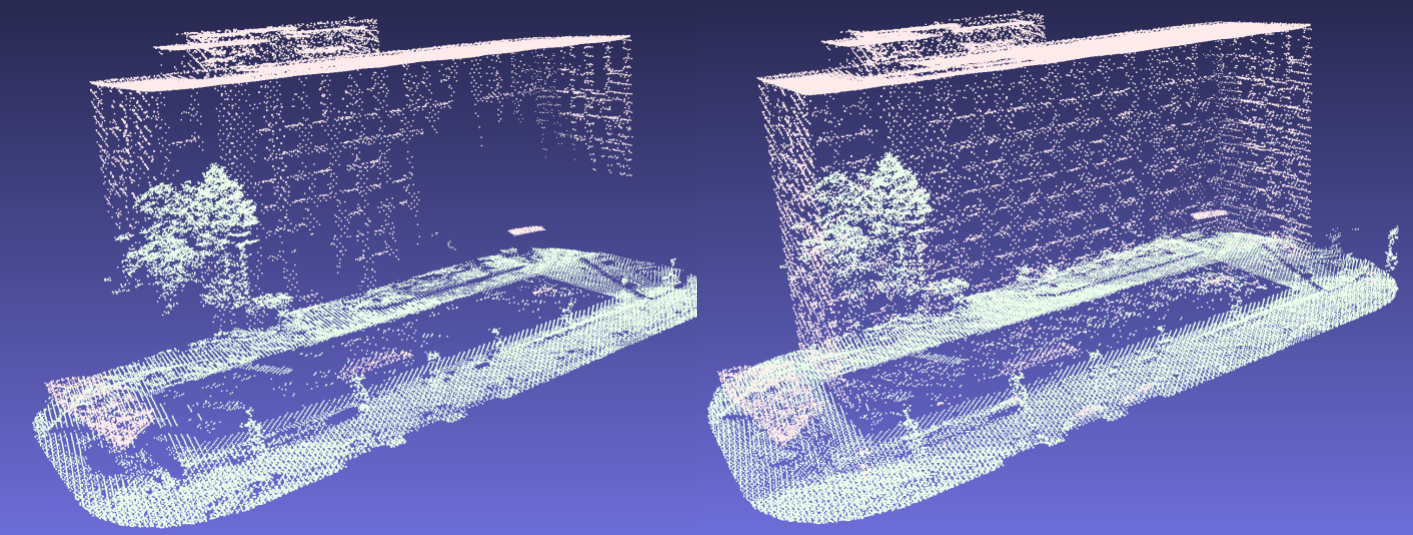
\includegraphics[width=\linewidth]{orca_house.png}
        \caption{Ground truth (left) of labelled data, and merged segmentation (right) of the labelled data and unlabelled data.}
        \label{fig:full-segmentation-results}
    \end{figure}

    \textbf{Limitations.} The model is occasionally unable to segment very large buildings, as seen in Figure~\ref{fig:large-building-segmentation-results}.
    This is due to the lack of context in the block, and the model being unable to extrapolate the local features of the building.
    Due to the significant variation in the size of buildings in the dataset, simply choosing a larger block size may not be sufficient to solve this issue.
    With the same number of points, a larger block size leads to increased sparsity in the input data. 
    But with a large number of points, smaller buildings may not have enough points overall to be classified effectively. 
    Such a trade-off is difficult to resolve, and so the model is unable to segment the roofs of some very large buildings.
    This is not a significant limitation, as it is typically in the walls where large chunks of the building are unlabelled in the original point cloud.
    As seen in Figure~\ref{fig:large-building-segmentation-results}, the walls are still classified effectively.
    This issue can be somewhat mitigated in the downstream task by taking the union of the learned building points and the points already classified as buildings.

    \begin{figure}
        \centering
        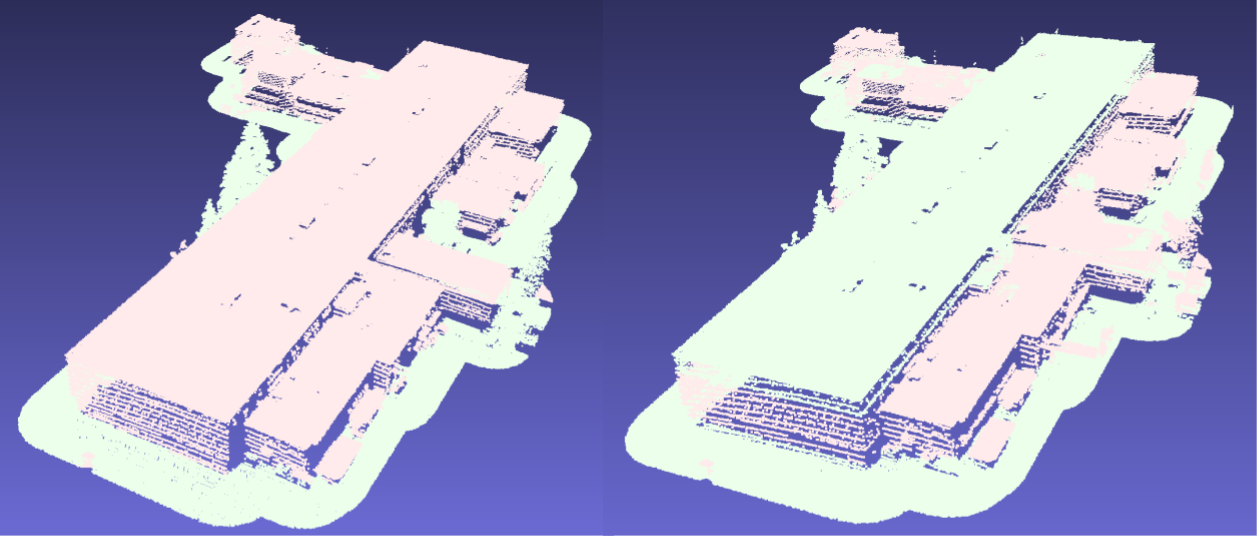
\includegraphics[width=\linewidth]{large_building_classification.png}
        \caption{Semantic segmentation of a very large building, where the model incorrectly labels the roof as non-building.}
        \label{fig:large-building-segmentation-results}
    \end{figure}

    \subsection{Densification}\label{subsec:densification-results}

    \textbf{Qualitative Results.} The densification algorithm is performed on the union of the learned building points and the points already classified as buildings.
    Overall, the densification algorithm works well enough to upsample walls and roofs, as seen in Figure~\ref{fig:densification-results}.

    \textbf{Limitations.}
    Inherent limitations in the SAPCU algorithm lead to the densification algorithm being unable to create a high quality point cloud for downstream tasks.
    Given the algorithm was trained on watertight meshes, it does fully preserve the structure of holes in the mesh. Windows are thus not preserved effectively in the densification process.
    In Figure~\ref{fig:densification-results}, the densification algorithm is unable to preserve the windows in the building, and many of the windows are either smaller or no longer have their edges preserved effectively.
    Additionally, the noise caused by incorrect semantic segmentation is significantly amplified after upsampling. This leads to large artefacts in most of the densified buildings, as seen in Figure~\ref{fig:densification-results}.

    \begin{figure}
        \centering
        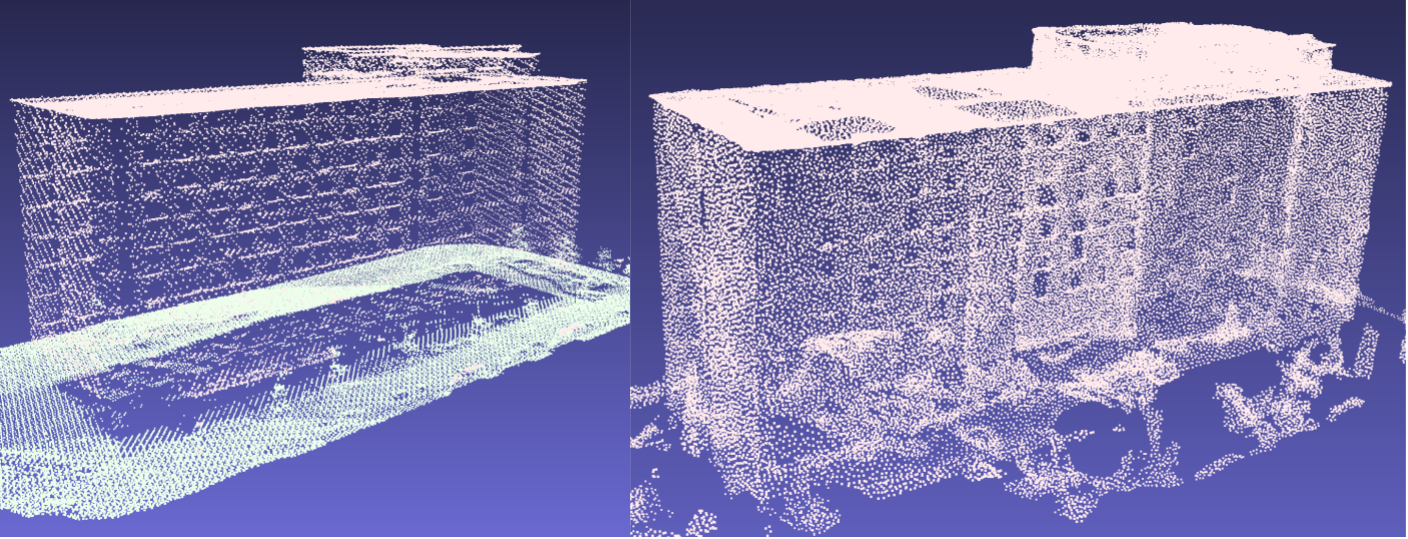
\includegraphics[width=\linewidth]{densification_results.png}
        \caption{Original labelled point cloud (left) and densification of the labelled point cloud (right). Though upsampling walls and roofs, the model amplifies noise from the segmentation task in the labelled point cloud.}
        \label{fig:densification-results}
    \end{figure}

    An additional drawback with the recursive algorithm is that it leads to differences in the density of the point cloud based on the median split. 
    The number of sampled points was chosen to be 2x the number of input points throughout the entire algorithm, however differences in overall density through this median split will be amplified.
    This is shown in Figure~\ref{fig:median-split}, where the densification algorithm is unable to upsample the building to the same extent throughout the building.

    \begin{figure}
        \centering
        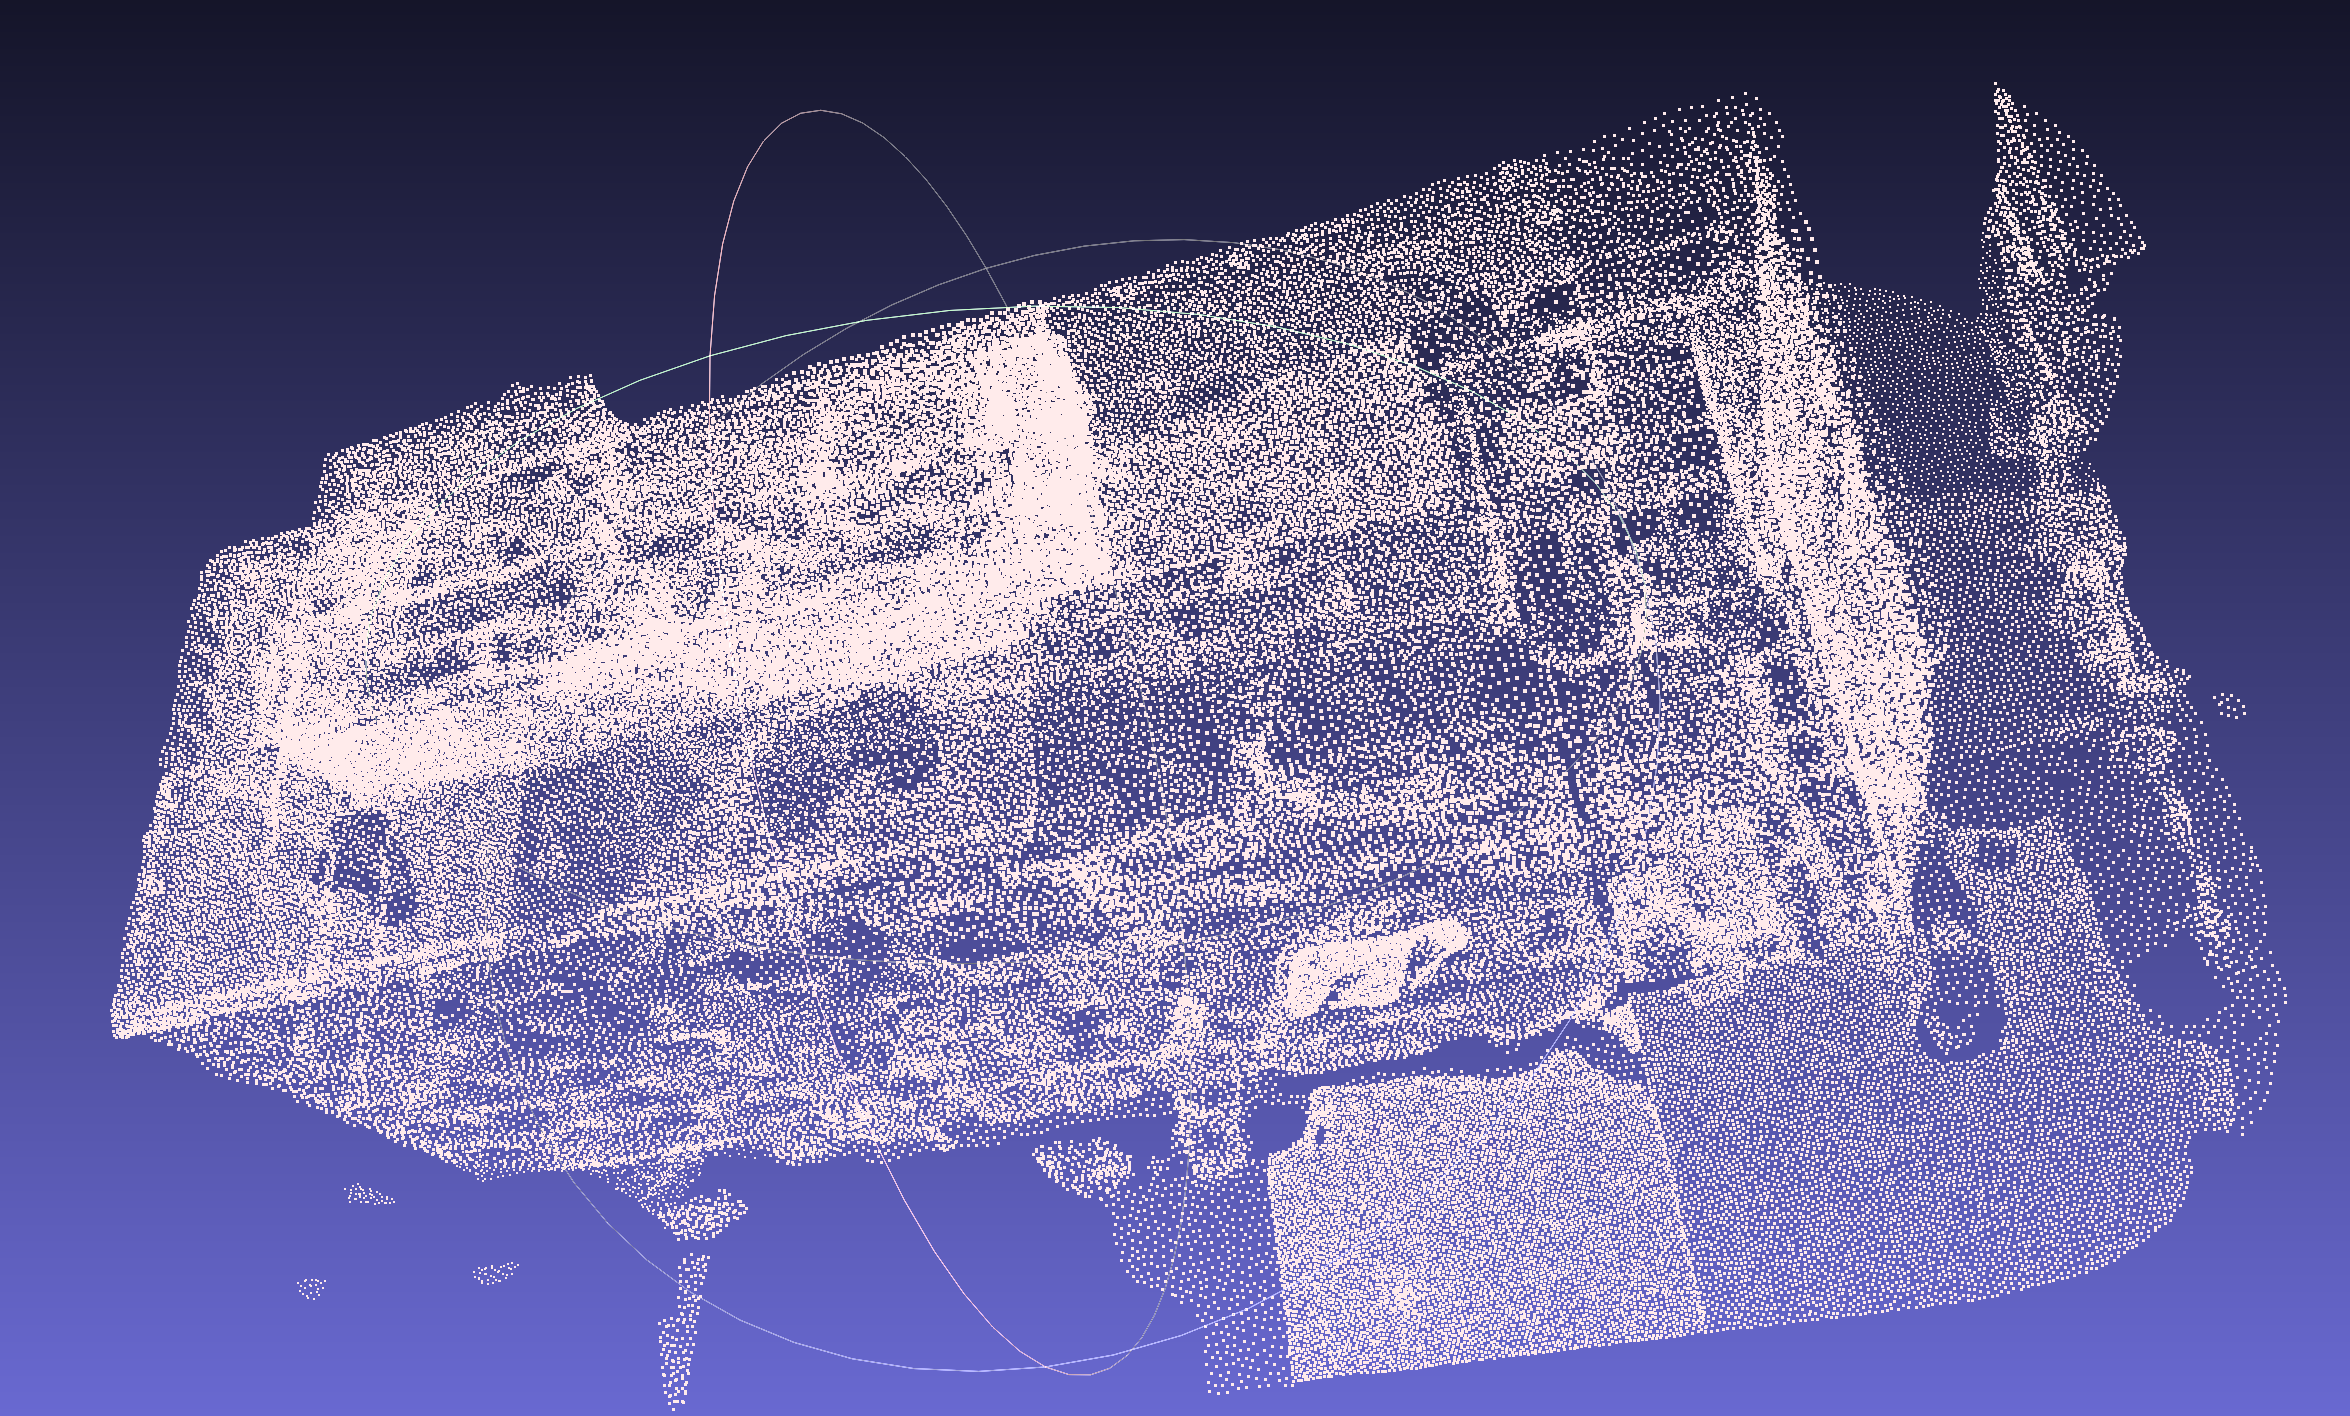
\includegraphics[width=\linewidth]{visible_split.png}
        \caption{Visible split along recursive median lines in the densified point cloud. Split lines are visible both in ground data and building data}
        \label{fig:median-split}
    \end{figure}

    \subsection{Planar Flattening}\label{subsec:planar-flattening-results}

    Due to time constraints, the planar flattening task is not implemented through code, so no results are yet available.
    Planar flattening is expected to reduce the noise in the voxelization process, and improve voxelization quality.
    It would also be useful to perform the planar flattening task on the non-densified point cloud to assess its effectiveness in improving the densification process.

    A full ablation study was not performed as a result of the planar flattening process being left for future work. 
    However, the planar flattening process is expected to improve downstream tasks, as it reduces noise in the point cloud and improves voxelization quality.

    \section{Conclusion}\label{sec:conclusion}

    LiDAR-DenseSeg represents an advancement in processing airborne LiDAR data for voxelization and mesh reconstruction. The framework's ability to segment, densify, and reduce variance in the point cloud results in a more accurate and detailed reconstruction of physical structures, particularly buildings. While the implementation showcases notable improvements in handling sparsity and noise in LiDAR data, certain limitations such as challenges in semantically segmenting very large buildings and densifying non-watertight meshes were identified. Future work can explore refining these aspects, potentially enhancing the framework's robustness and applicability, as well as continuation of the planar flattening task. Overall, LiDAR-DenseSeg stands as a promising solution for the accurate and efficient reconstruction of complex environments from LiDAR data.

    \section{Acknowledgements}\label{sec:acknowledgements}

    The dataloader for PointNet++ is somewhat based on the S3DIS dataloader in the PyTorch implementation of PointNet++~\cite{qi2017pointnet, PytorchPointnetPointnet2}.

    The recursive median SAPCU algorithm is an extension on the original implementation of the SAPCU architecture~\cite{sapcu}.

    \bibliographystyle{IEEEtran}
    \bibliography{LiDAR-DenseSeg}

\end{document}
